% !TEX root = presentation.tex
% \begin{frame}
%     \frametitle{Minkowski Sum}
%     \framesubtitle{Example}
%     \topskip0pt
% 	\vspace*{\fill}
%     \begin{center}
%     	\todo[inline]{Schermvullend plaatje}
% 	\end{center}
% 	\vspace*{\fill}
% 	\mbox{\tiny{Image adapted from: \url{http://allenchou.net/2013/12/game-physics-collision-detection-csos-support-functions/}}}
% \end{frame}

\plain{
	% 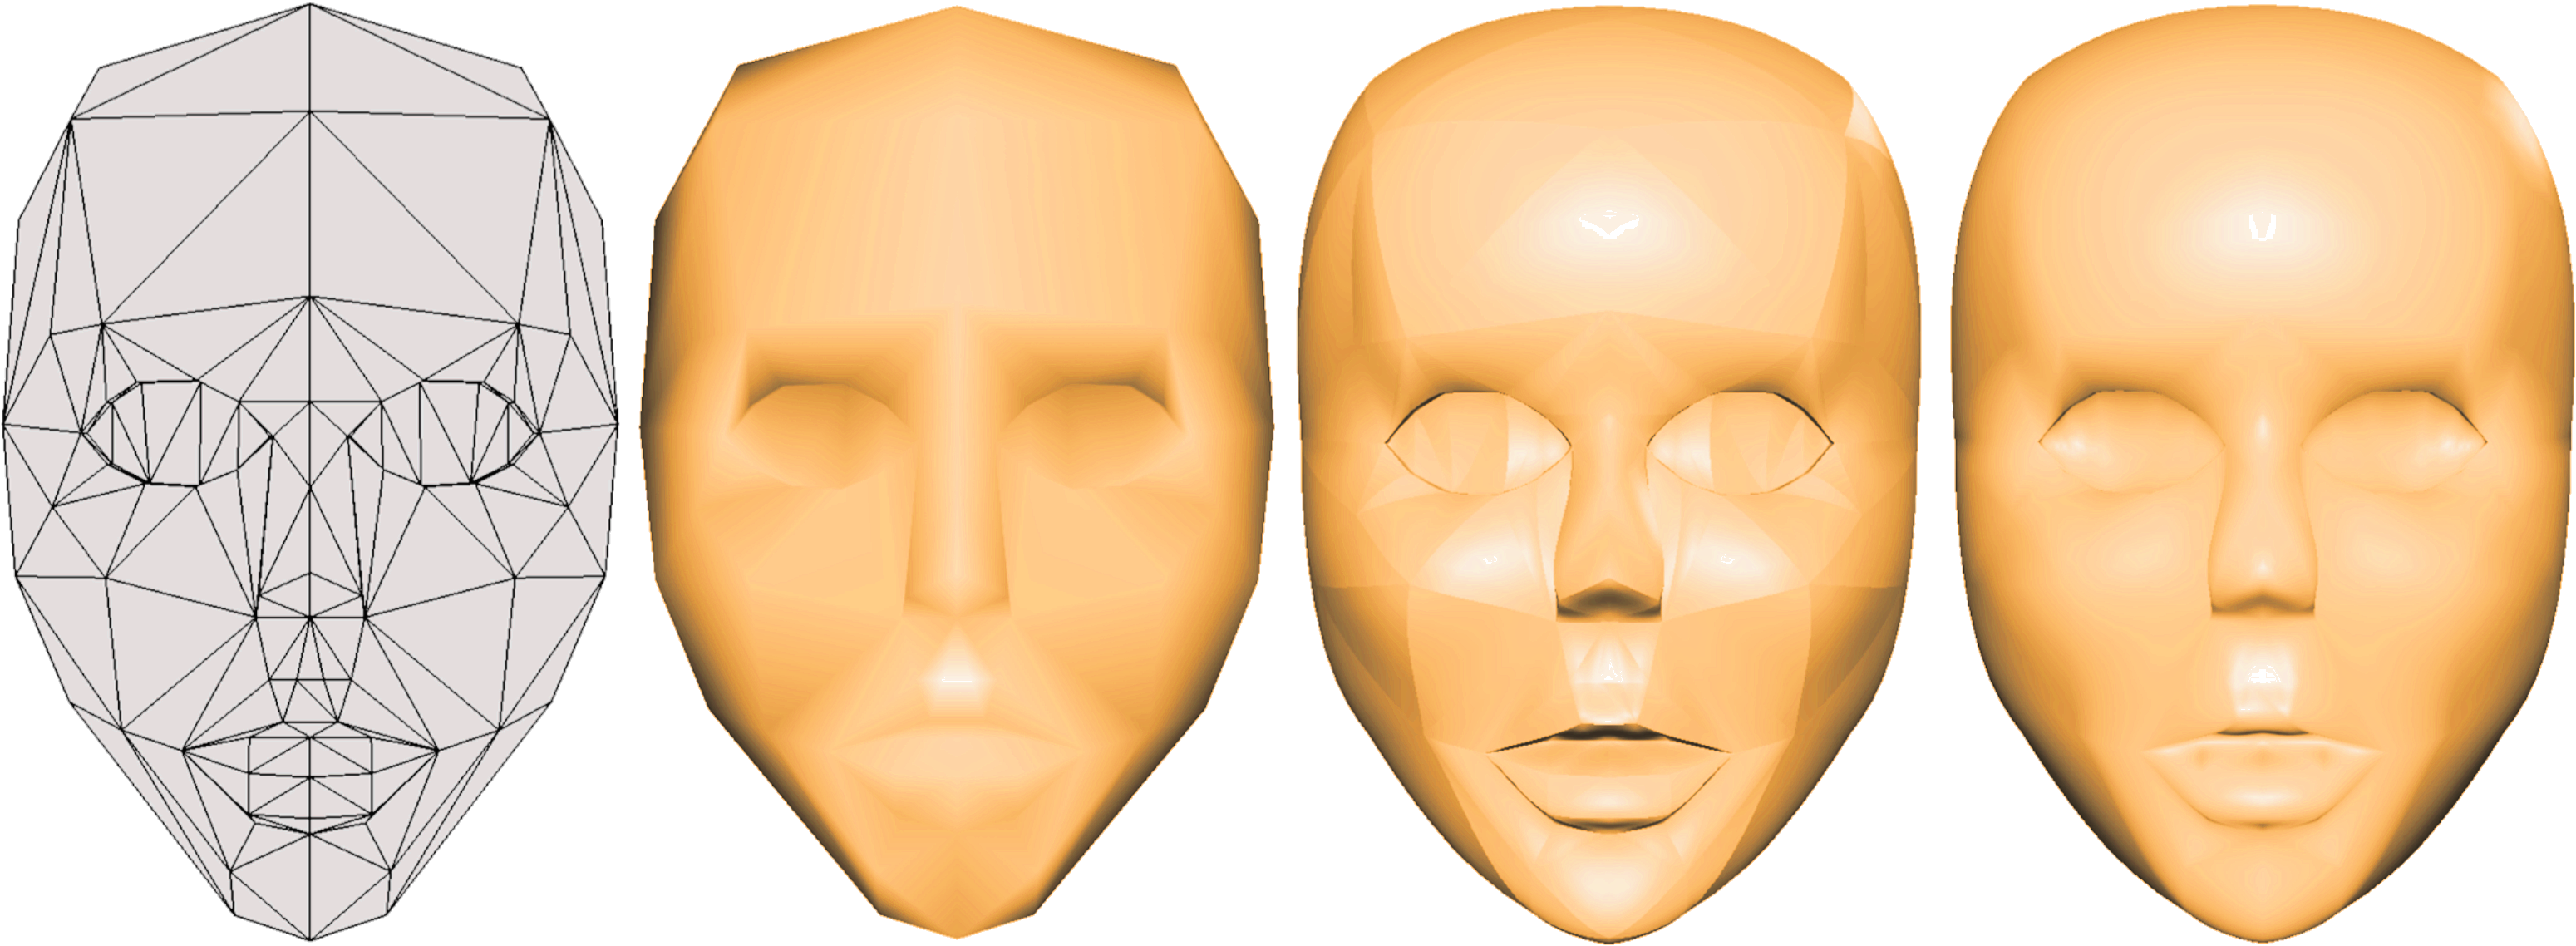
\includegraphics[width=\textwidth]{img/00_results_orange.png}
	\begin{figure}
		\centering
		\begin{subfigure}{0.24\textwidth}
			\centering
			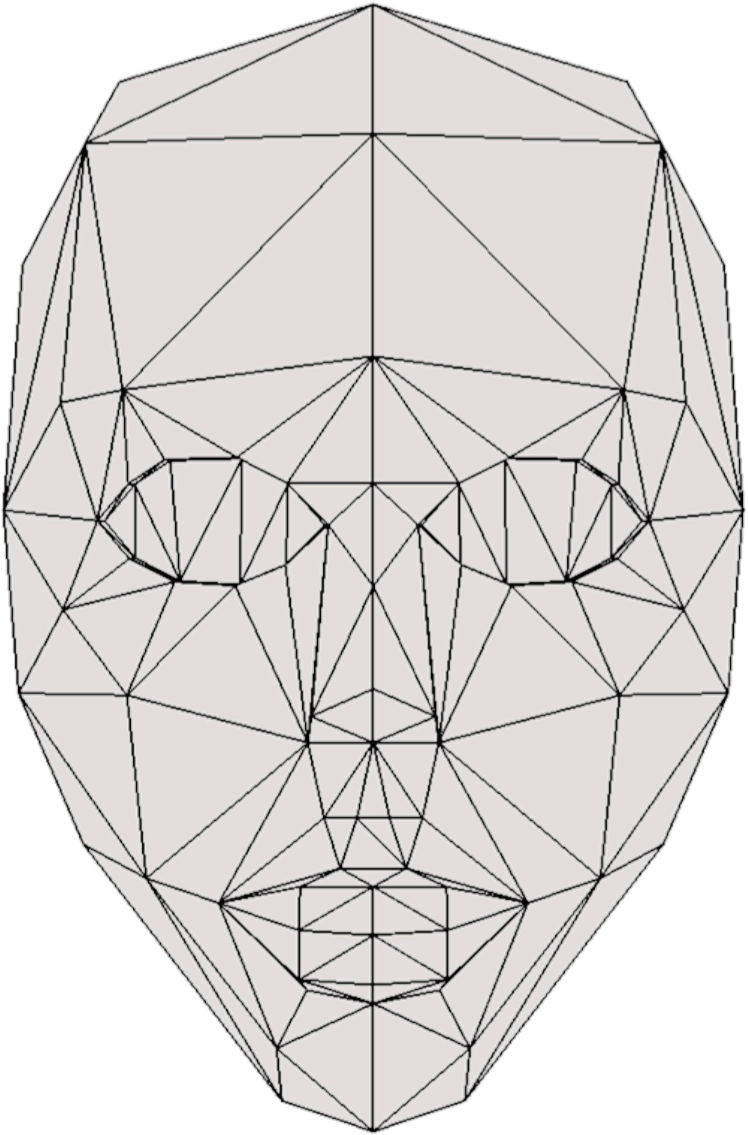
\includegraphics[width=\textwidth]{./img/00_results_orange_1.png}
			\caption{Input triangulation}
		\end{subfigure}
		\begin{subfigure}{0.24\textwidth}
			\centering
			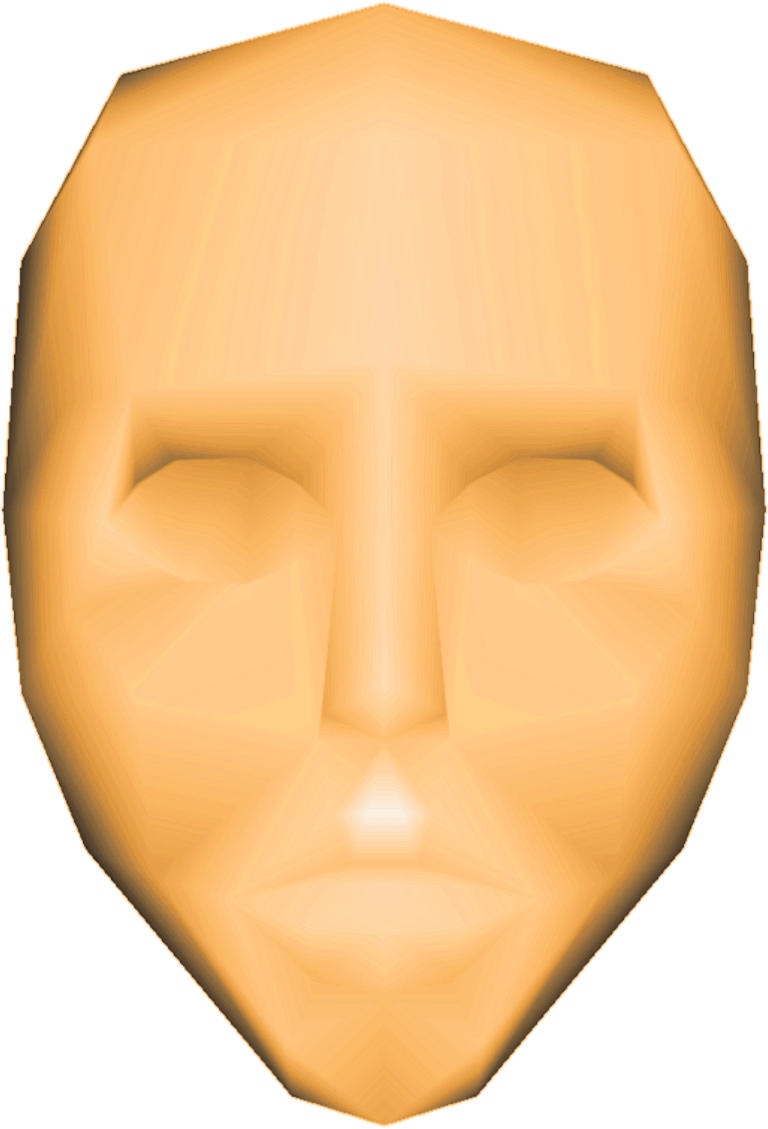
\includegraphics[width=\textwidth]{./img/00_results_orange_2.png}
			\caption{Gouraud shading}
		\end{subfigure}	
		\begin{subfigure}{0.24\textwidth}
			\centering
			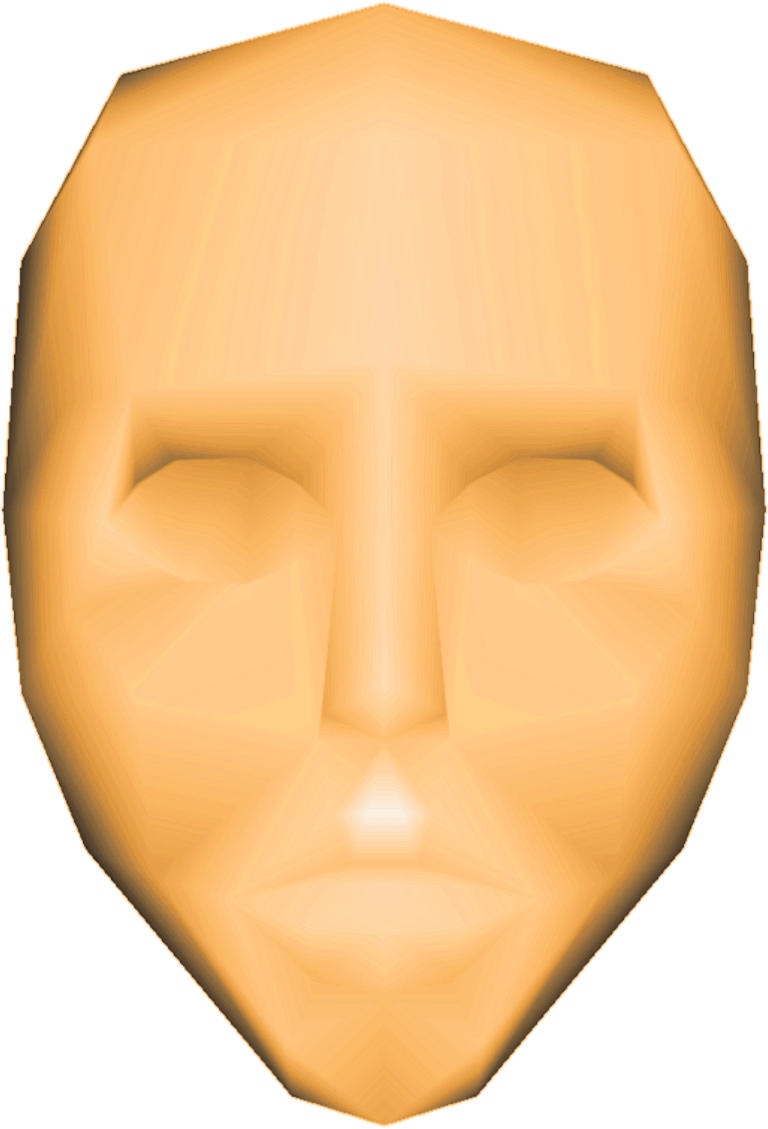
\includegraphics[width=\textwidth]{./img/00_results_orange_3.png}
			\caption{Geometry component}
		\end{subfigure}	
		\begin{subfigure}{0.24\textwidth}
			\centering
			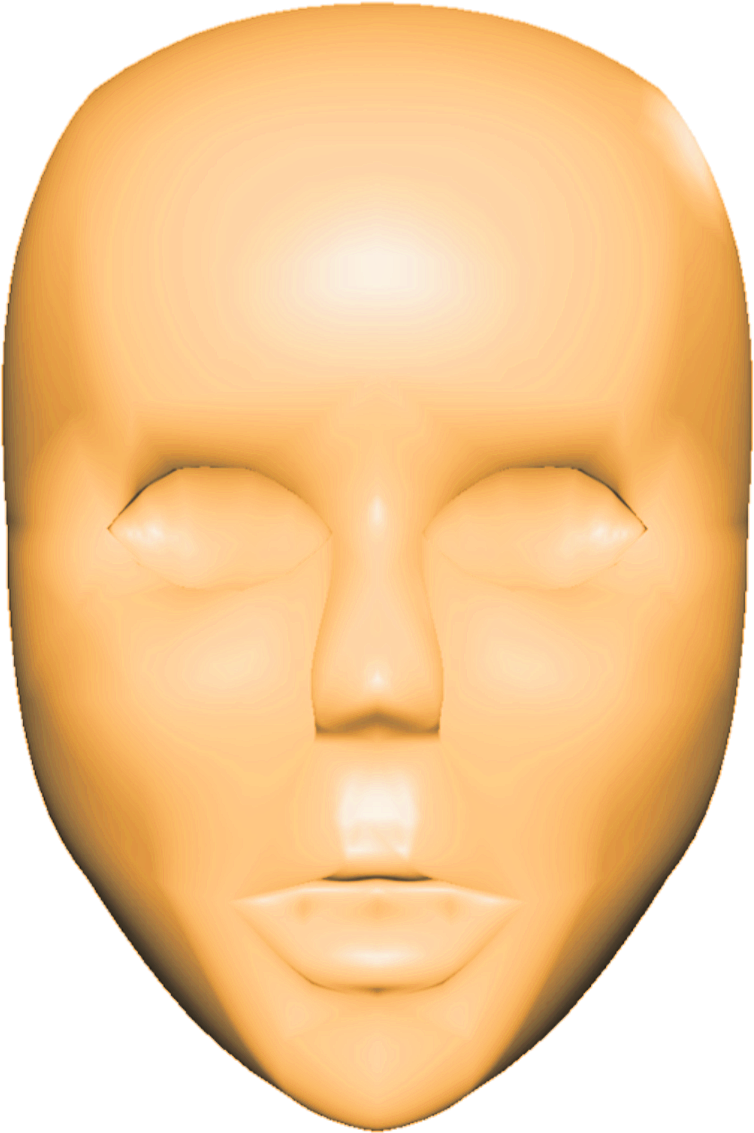
\includegraphics[width=\textwidth]{./img/00_results_orange_4.png}
			\caption{PN Triangle}
		\end{subfigure}	

		\caption{}
	\end{figure}
}
